\documentclass[]{article}
\usepackage{siunitx} % si eenheden
\usepackage{hyperref}					% maak PDF van de thesis navigeerbaar
\usepackage{url}
\usepackage[toc,acronym,xindy]{glossaries}%voor afkortingen
\usepackage{amsmath}
\usepackage[official]{eurosym} % om euro symbool te kunnen gebruiken
\usepackage{graphicx}
% MFA: zet zoekpad voor figure
\graphicspath{{fig/}}
\usepackage{float}                      % De optie H voor de plaatsing van figuren op de plaats waar je ze invoegt. bvb. \begin{figure}[H]
%opening
\title{Cosy Cafeteria: Masterplan}
\author{ Robin Van de Poel\and Arthur Van den Storme\and Tobias Cromheecke\and Thomas Feys 
}

\begin{document}

	\maketitle
	
	\section{Concept}
	To improve the experience of the students in the cafeteria, an embedded system will be developed to gather a variety of data. This data will then be display to the students through an online medium such as a website. The main focus will be to gather information about the amount off people that are in the cafeteria. There are two main goals. The first goal is to display the estimated waiting time to get a meal to the students. Secondly the amount of available seats will be tracked and displayed to the students. Next to this some additional information will be gathered. The temperature, air-quality and sound level will be monitored to give the student a general idea about the conditions in the cafeteria. This way the student can gauge if the cafeteria is suitable to study in at a certain moment. 

	\section{Specifications}
	\subsection{Functional specifications}
	\begin{itemize}
		\item Monitor the available seats
		\item Monitor the queue to get a meal
		\item Display the data to the students
		\item Energy provision for 1 semester (4-5 months)
		\item Wireless coverage over the entire campus
		\item Measure new data every 10 minutes
		\item Send the data to the online medium every hour 
		\item If the data changes with a large amount (needs to be specified) update the online medium sooner
	\end{itemize}

	\subsection{Other technical specifications}
	\begin{itemize}
		\item Enclosure: 10 x \SI{10}{\centi\meter}
		\item Easy deployment: the node must be easy to attach and detach from the sealing
		\item Must be easy to recharge (Wireless or via USB)
		\item Light weight: \SI{300}{\gram} (so it wont detach from the sealing)
	\end{itemize}
	
	\subsection{Non-technical specifications}
	\begin{itemize}
		\item Cost: \euro{??}
		\item The data should be easy accessible to the students
		
	\end{itemize}
	\subsection{Situation sketch}
	\begin{figure}[!ht]
		\centering
		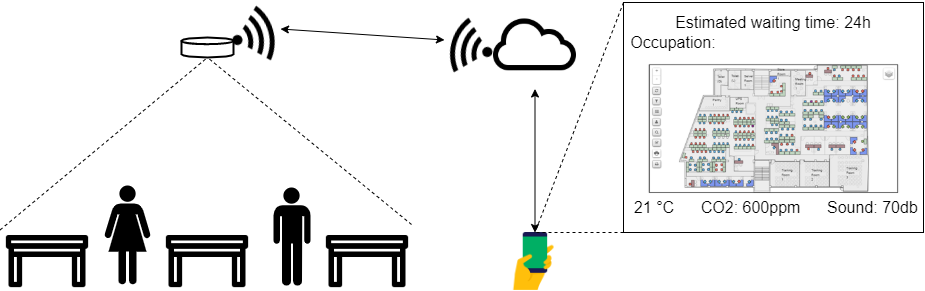
\includegraphics[width=1\linewidth]{situation.png}
		\caption{Situation sketch}
		\label{fig:situation}
	\end{figure} 
	
	\section{System architecture}

	\section{Responsibilities}
	\subsection{Technical:}
	\begin{itemize}
		\item Power system (Battery, under and overcharge protection, voltage converters,...): Tobias
		\item Communication system: Thomas and Tobias
		\item PCB integration: Arthur
		\item Sensors: Robin
		\item Software integration: Thomas
		\item Online dashboard to display data: Arthur
		\item Enclosure: Robin
	\end{itemize}

	\subsection{Non-technical: }
	\begin{itemize}
		\item Time manager: Robin
		\item Project manager: Thomas
		\item Documentation/Report: Tobias
		\item Presentation: Arthur
	\end{itemize}

	\section{Milestones}
	
\end{document}
